\section{Others}

\subsection{Performance Metrics} 

Para medir el performance de un modelo de \textit{Machine Learning} ya sea en problemas de clasificación o regresión, es posible utilizar distintas métricas de acuerdo a lo que nos importa medir en cada situación. 

\subsubsection{Classification Metrics}

\begin{figure}[H]
    \center
    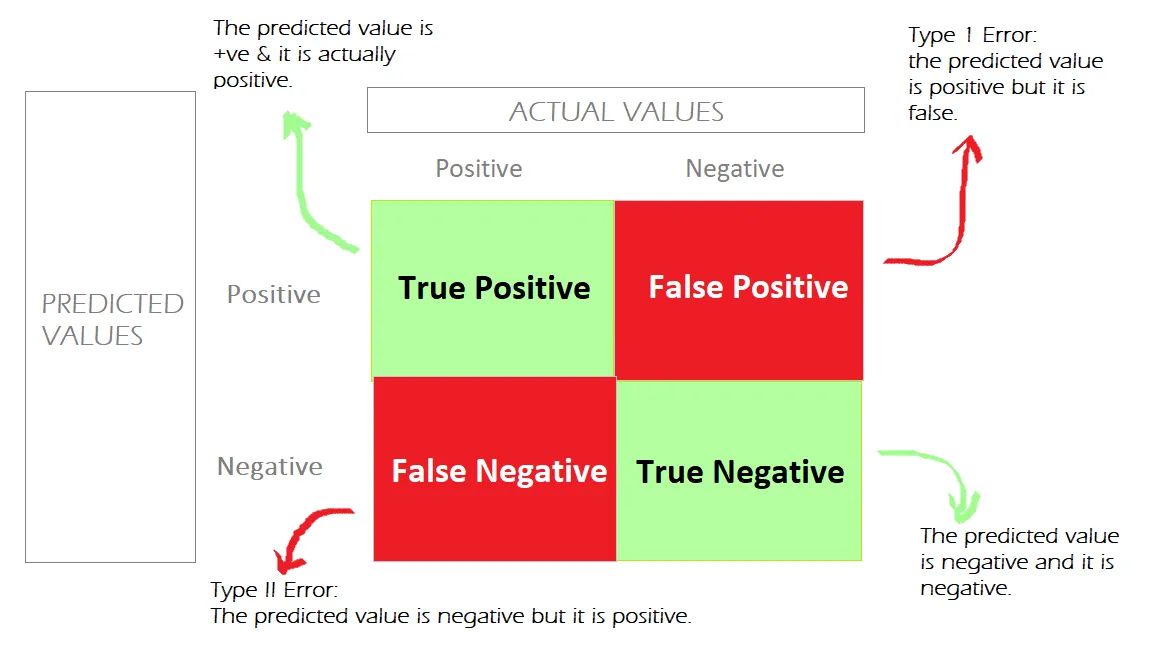
\includegraphics[scale=0.25]{notebooks/Others/img/confusion_matrix_diagram.png}
    \caption{Confusion Matrix Diagram}
\end{figure}

En las métricas para problemas de clasificación, podemos encontrar
\begin{enumerate}
    \item \textbf{Accuracy:} Se define como el total de aciertos positivos y negativos sobre el total de predicciones. 
    $$ 
    \text{Accuracy} = \frac{TP + TN}{TP + TN + FP + FN}
    $$
    \item \textbf{Precision:} Este es el porcentaje de identificaciones positivas correctas en el total de identificaciones positivas. 
    $$
    \text{Precision} = \frac{TP}{TP + FP}
    $$
    \item \textbf{Recall: } Este es el porcentaje de identificaciones positivas correctas en el total de datos positivos. 
    $$ 
    \text{Recall} = \frac{TP}{TP + FN}
    $$
    \item \textbf{F1 - Score: } Esta métrica es la media armónica entre la precisión y el recall. 
    $$ 
    F_{1} = \frac{2}{\frac{1}{\text{precision}} + \frac{1}{\text{recall}}} = 2 \frac{\text{precision} \cdot \text{recall}}{\text{precision} + \text{recall}}
    $$
    Si alguna de las métricas tiene una mayor importancia dado el contexto del problema, podemos amplificarla por un valor $\beta$ de la siguiente forma
    $$ 
    F_{\beta} = (1 + \beta^2) \frac{\text{precision} \cdot \text{recall}}{\beta^2 \cdot \text{precision} + \text{recall}}
    $$
    Es decir, el recall es $\beta$ veces más importante que la precisión. 
\end{enumerate}

En problemas de clasificación binario, definir si un score se asigna al label positivo (1) o negativo (0) depende de un umbral (threshold) que se puede definir en base a qué métrica queremos optimizar. Lo anterior da origen a la curva \textit{Precision - Recall}





\subsection{Bias vs Variance}

El dilema de \textit{Bias vs Variance} describe la relación entre la complejidad del modelo, la precisión de las predicciones y cómo éste se comporta al predecir datos nunca antes vistos. El error estimado de una predicción viene dado en términos generales por 
$$
\text{Expected Error} = (\text{Bias})^2 + \text{Variance} + \text{Irreductible Error}
$$
Así, un modelo que crece en complejidad reducirá su bias pero aumentará su varianza (extremo: overfitting) y a la vez, reducir la complejidad permitirá generalizar mejor reduciendo la varianza pero aumentando el bias (extremo: underfitting). 

\begin{figure}[H]
    \center
    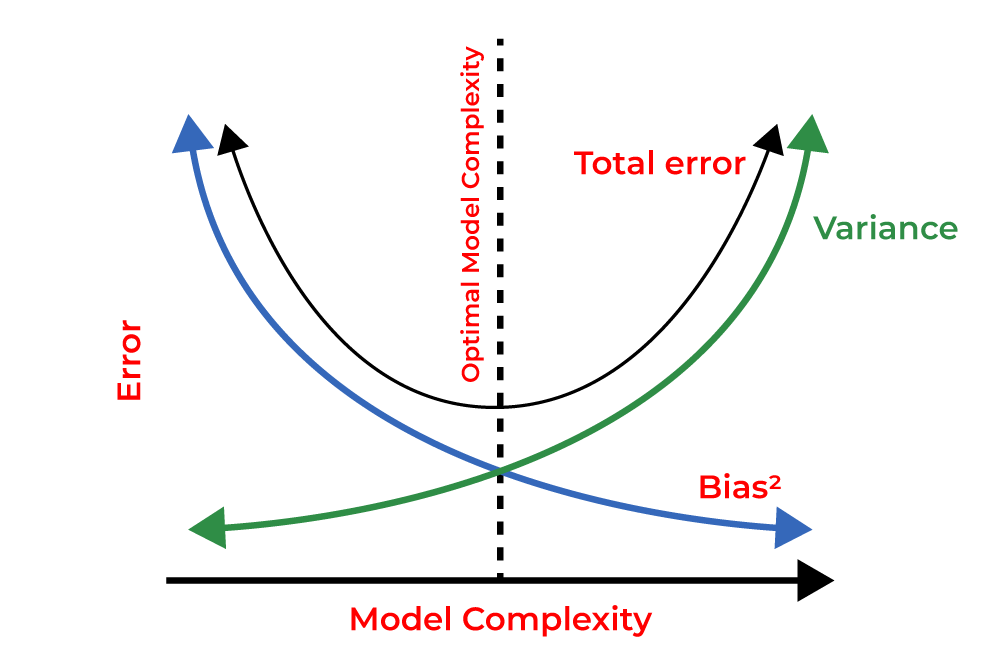
\includegraphics[scale=0.3]{notebooks/Others/img/bias_vs_variance.png}
    \caption{Bias vs Variance Diagram}
\end{figure}

\subsection{Oversampling and Undersampling}

\subsection{Random Noise Feature Importance}

\subsection{SHAP Values}
\label{subsec:shap_values}

El SHAP values (\textit{SHapley Additive exPlanations}) es un algoritmo modelo-agnóstico basado en teoría de juegos que permite \textbf{interpretar las predicciones}, la importancia de las variables y su impacto.

\begin{figure}[H]
    \center
    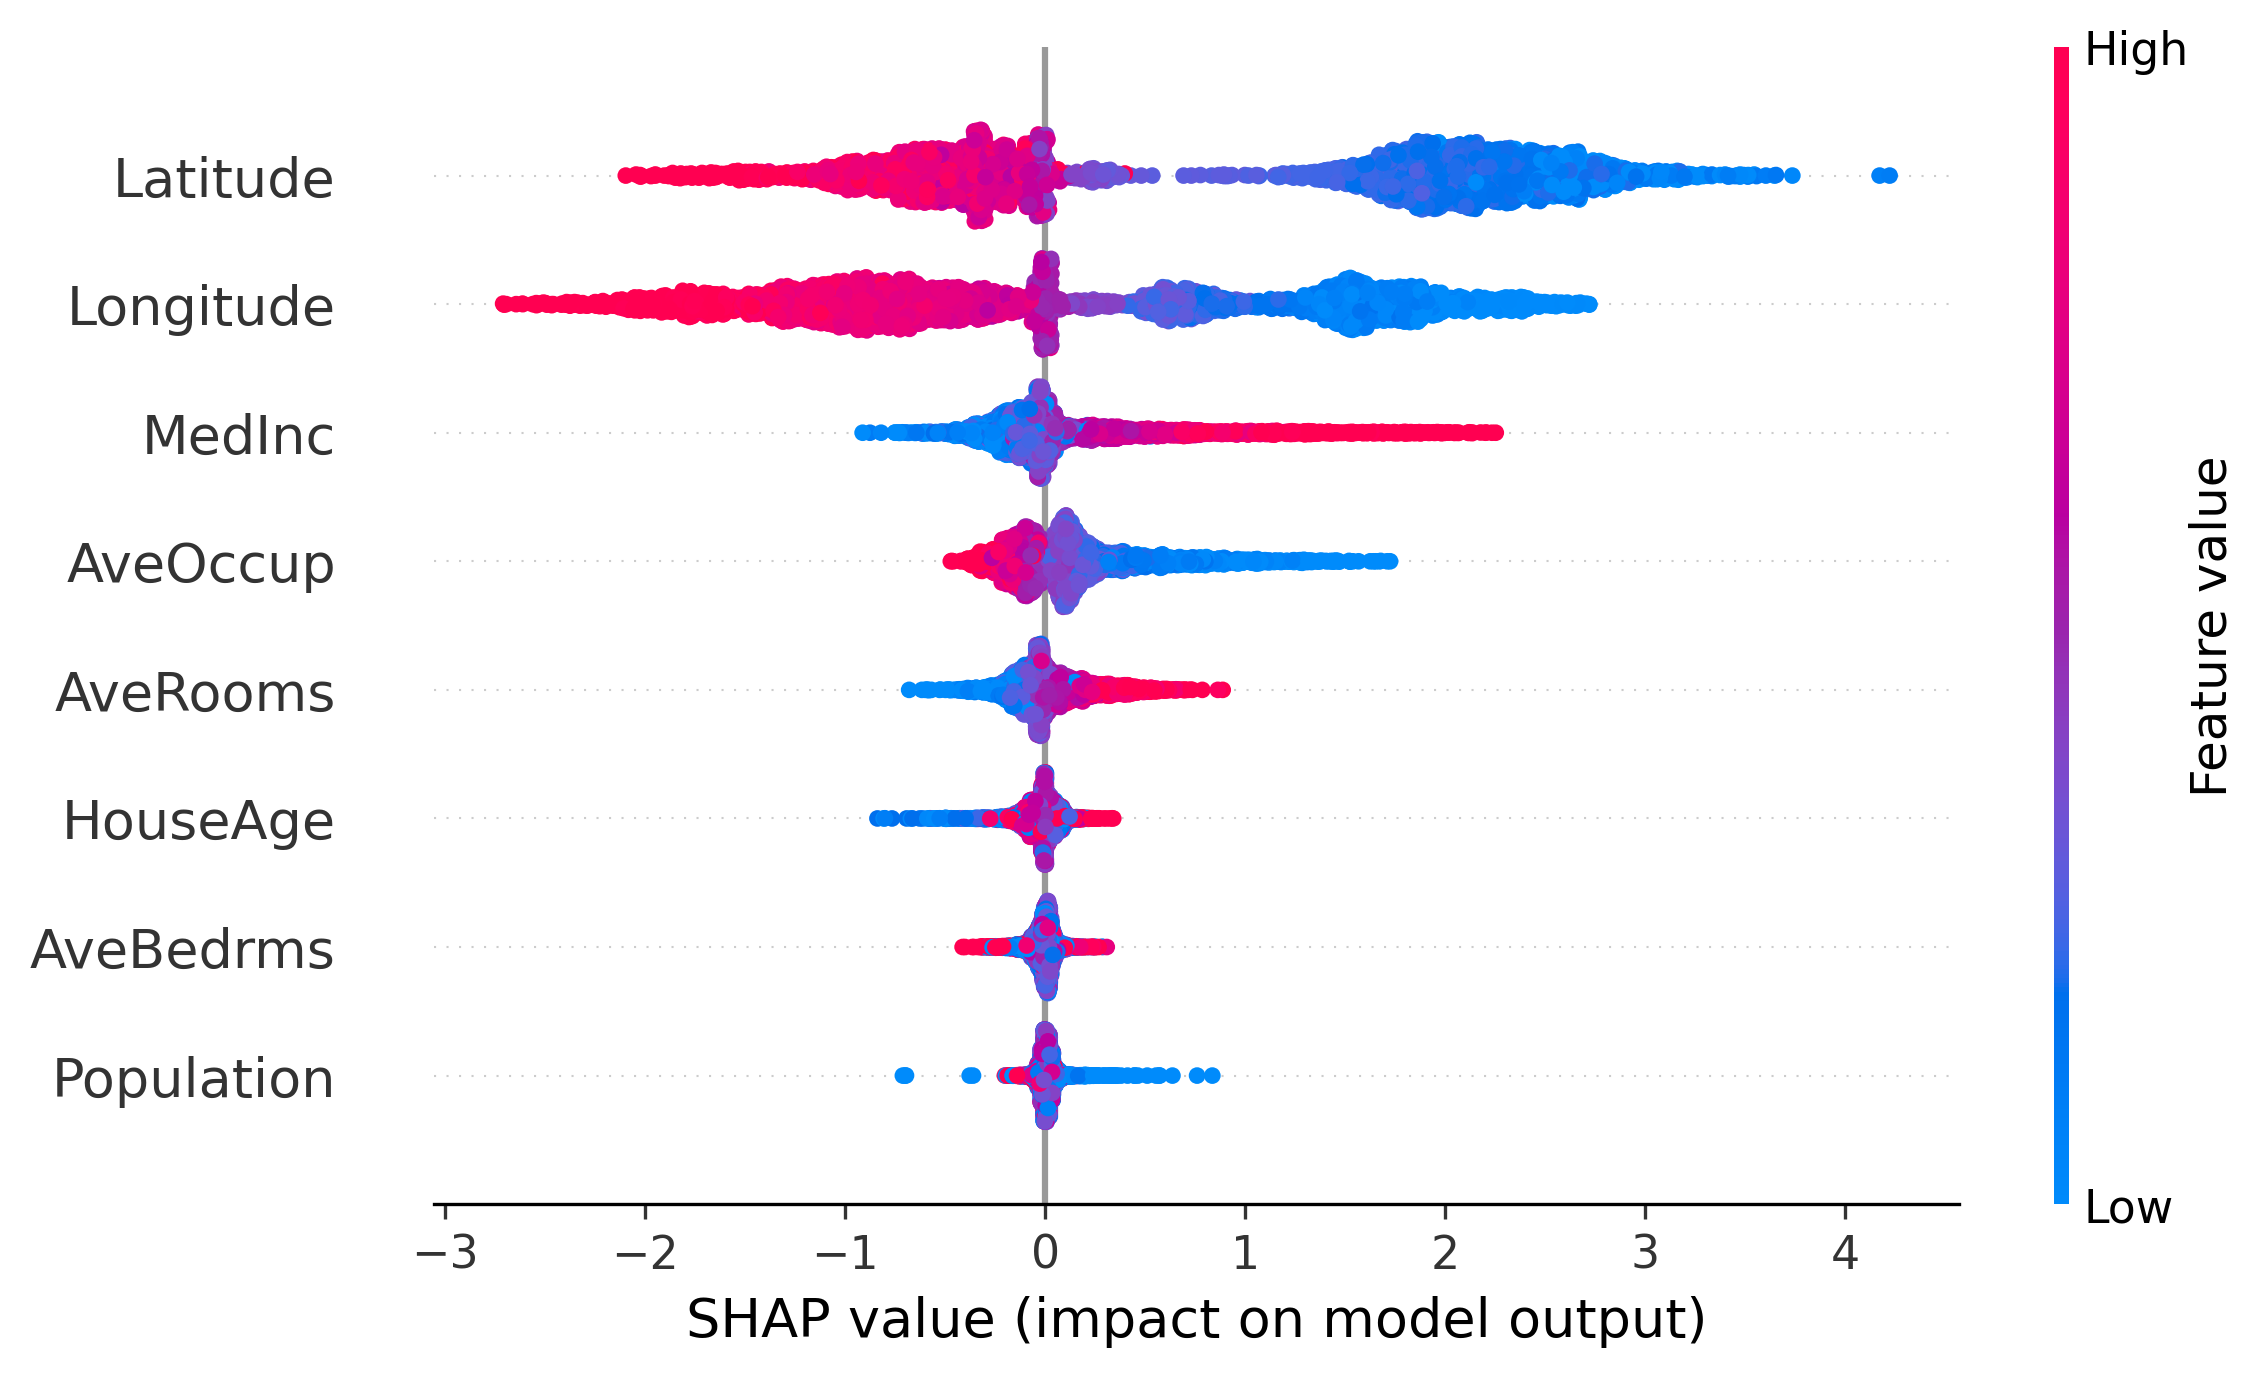
\includegraphics[scale=0.55]{notebooks/Others/img/shap_values_example.png}
    \caption{SHAP Values Example}
\end{figure}

\subsection{Outlier Detection}

La detección de outliers es la práctica de encontrar \textbf{datos anómalos} o fuera de distribución en un dataset. Es de suma importancia para la construcción de modelos de fraude o para mejorar el performance de modelos sensibles a outliers.

\begin{figure}[H]
    \center
    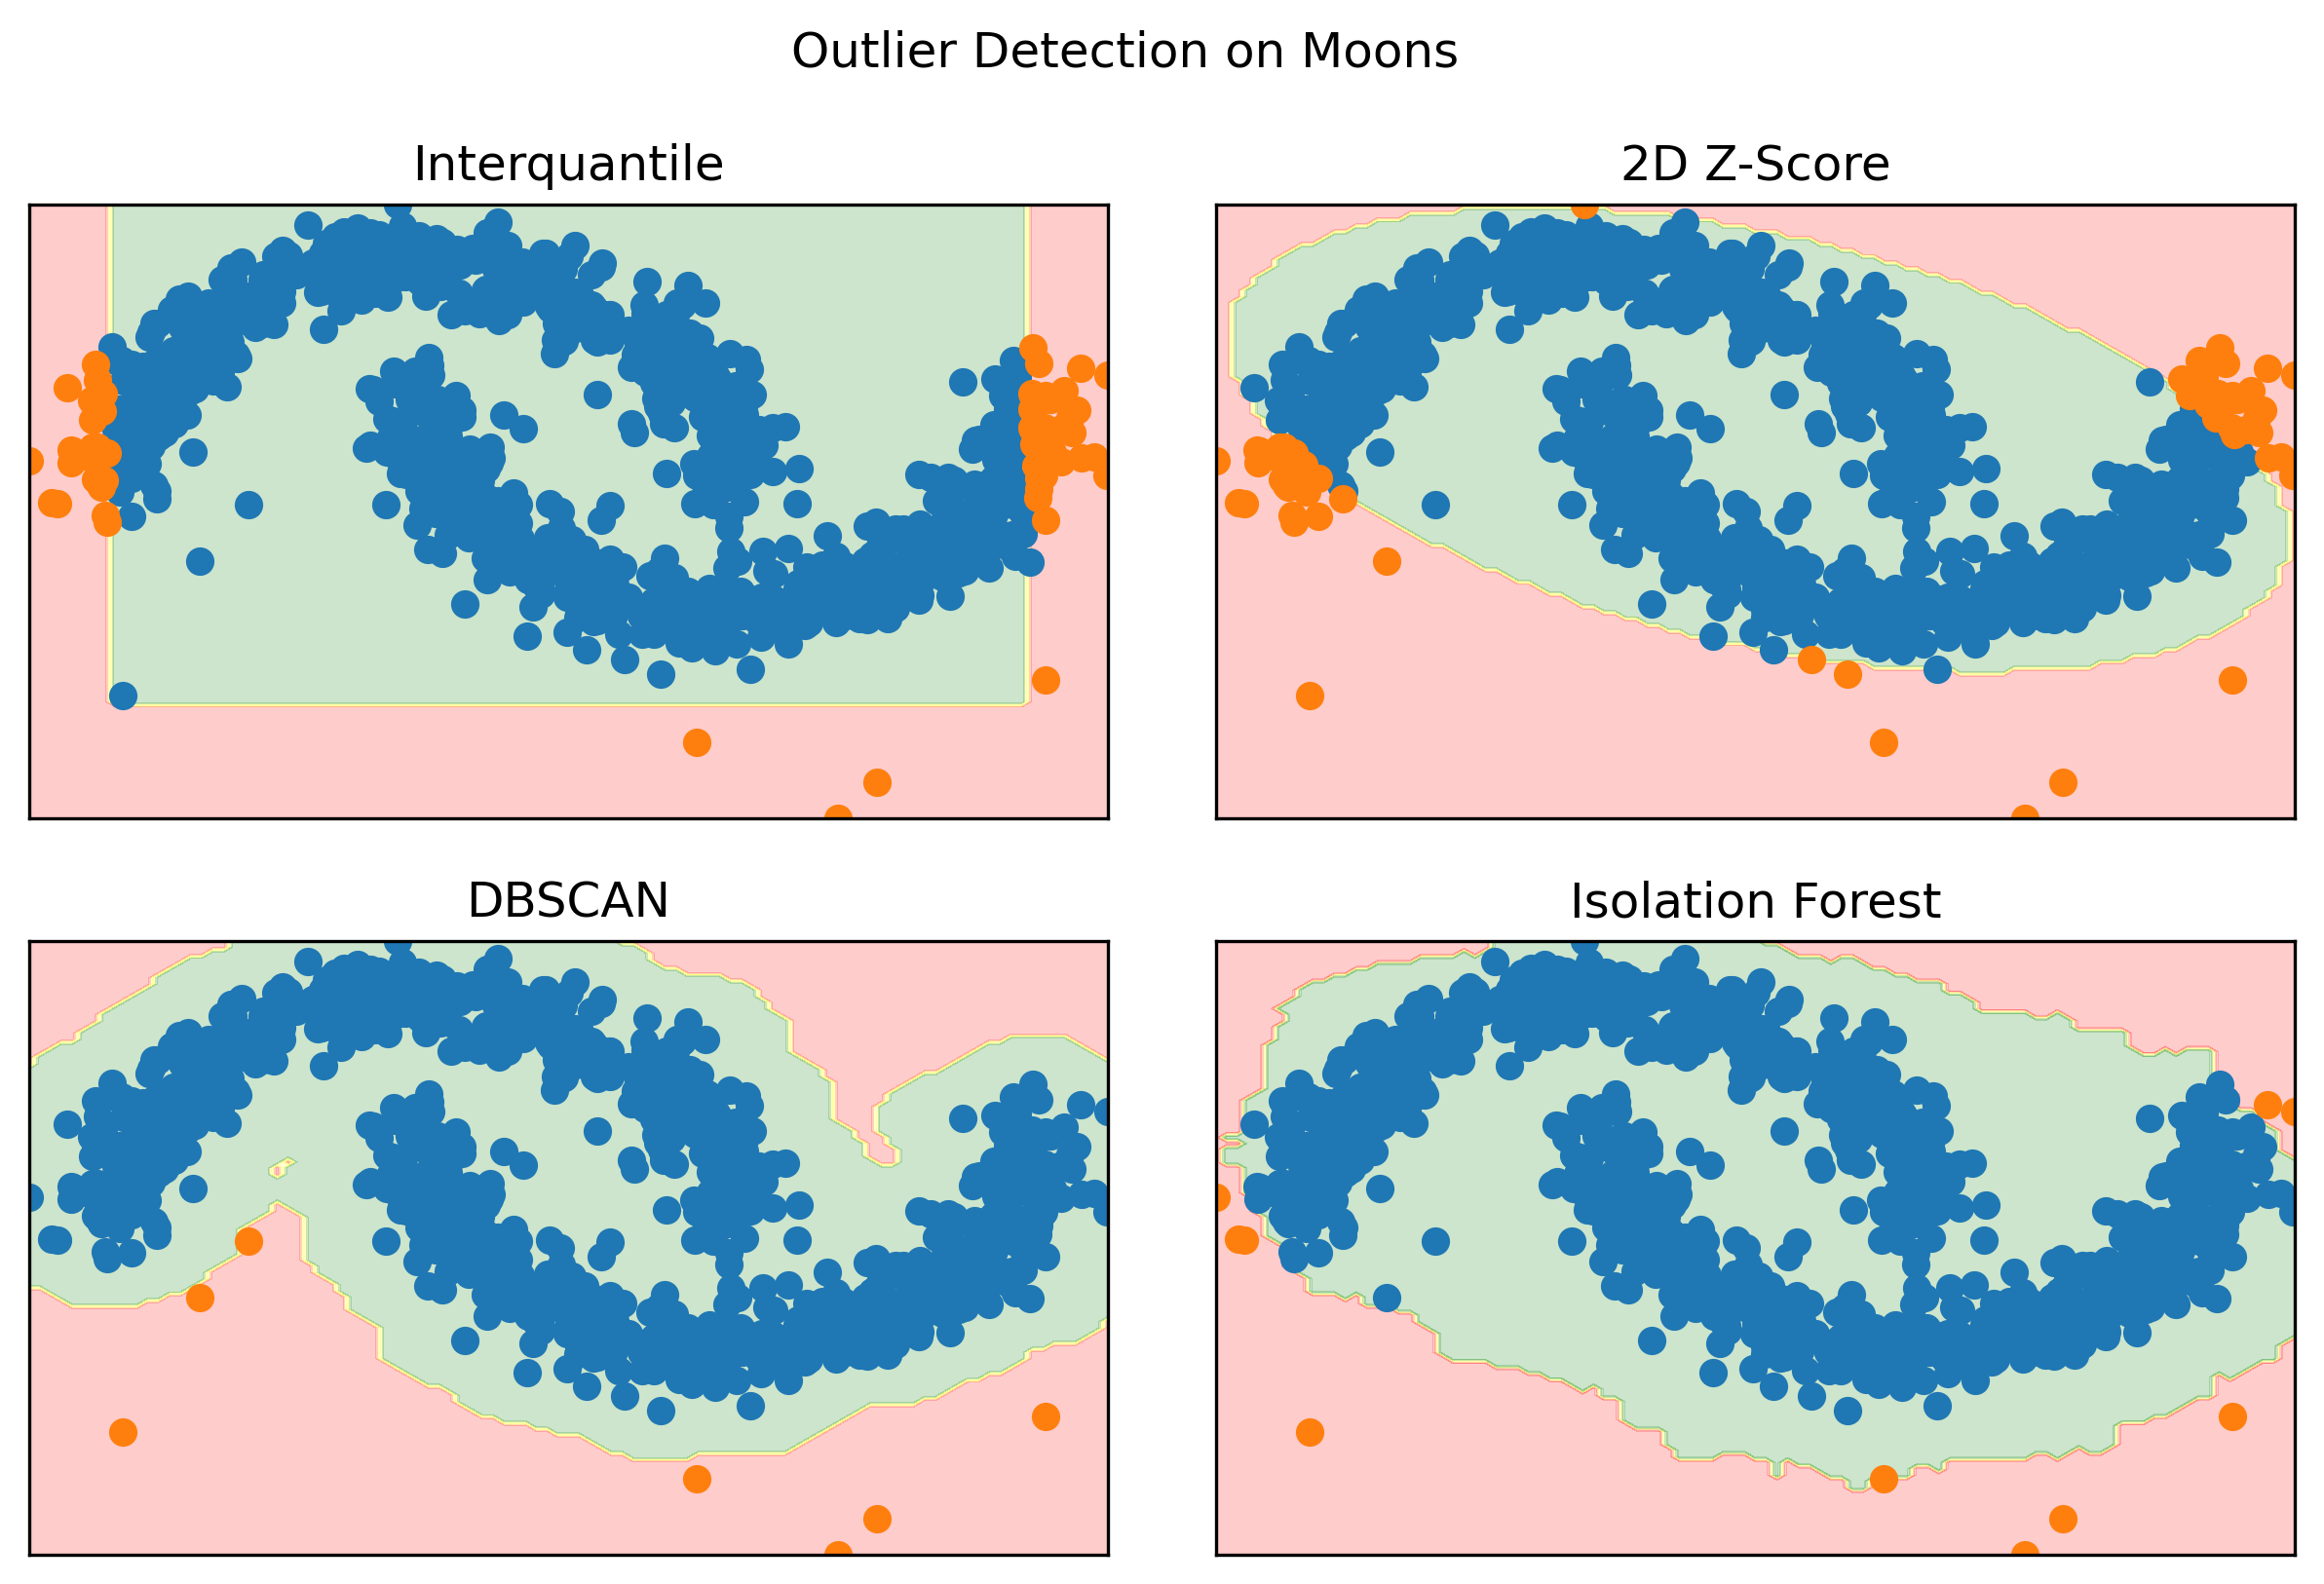
\includegraphics[scale=0.55]{notebooks/Others/img/outlier_detection.png}
    \caption{Outiler Detection Contour Plot}
\end{figure}

\subsubsection{Interquantile Range}

Definimos el \textit{Interquantile Range} IC como la diferencia entre el percentil 75 y el percentil 25. Es decir, 
$$ 
IC = Q_3 - Q_1
$$
En este caso, los outliers serán aquellos datos $x_i$ tal que 
$x_i \geq Q3 + I_{\text{range}}IC$ o bien $x_i \leq Q1 - I_{\text{range}}IC$
donde $ I_{\text{range}}$ permite controlar el porcentaje de outliers que se espera encontrar. (Equivalencia en distribución normal $I_{\text{range}} = 1.5 \approx Z_{\text{value}} = 2.69$).

Notar que en esta metodología no se asume normalidad en la distribución de los datos. 

\subsubsection{Z - Score}

Cuando los datos siguen una distribución normal, se pueden considerar como outliers aquellos datos $x_i$ que cumplen 
$$\left | \frac{x_i - \mu}{\sigma}\right | \geq Z_{\text{value}}$$

Para los casos con más de una feature (multidimensional), se puede extender esta definición utilizando la \textbf{distancia de Mahalanobis} definida como 
$$
D = \sqrt{(x_i - \mu_i)^{\top}\Sigma^{-1}(x_i - \mu_i)}
$$
Donde $\Sigma$ es la matriz de covarianza y $\mu_i$ el vector de media. 

\subsubsection{DBSCAN}

Los datos que no cumplan el mínimo de vecinos a distancia menor de $\epsilon$ son considerados por DBSCAN como outliers.

\subsubsection{Isolation Forest}

El algoritmo de \textit{Isolation Forest} selecciona de manera aleatoria una feature y un corte aleatorio entre el mínimo y el máximo valor presente en esa feature. Esto es repetido múltiples veces hasta aislar cada uno de los puntos.

Este algoritmo iterativo, puede ser representado en el siguiente diagrama:

\begin{figure}[H]
    \center
    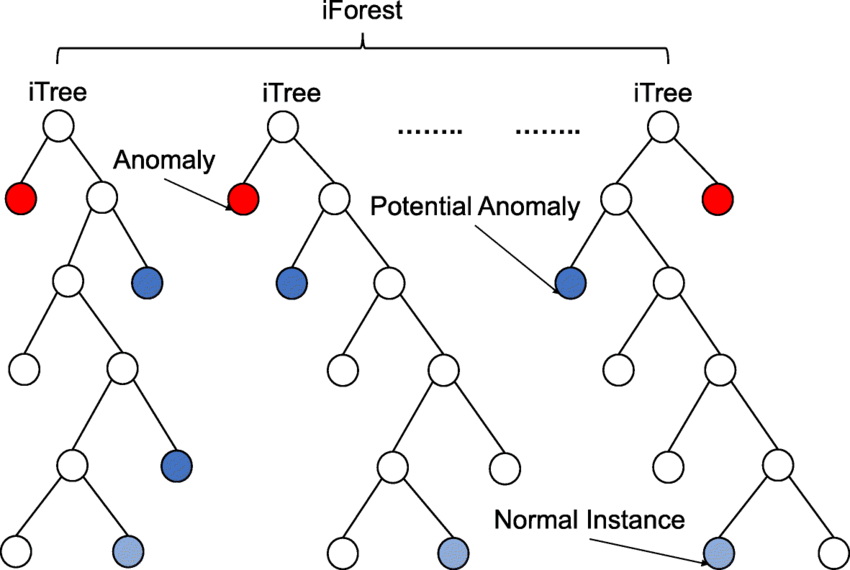
\includegraphics[scale=0.3]{notebooks/Others/img/isolation_forest_diagram.png}
    \caption{Isolation Forest Diagram}
\end{figure}

Los puntos que en promedio, requieren \textbf{menos divisiones para ser aislados}, son los que el algoritmo considera como potenciales datos anómalos (outliers).

\subsection{Cross-Validation Techniques}

El \textit{Cross-Validation} es un método que permite evaluar el rendimiento de un modelo de \textit{Machine Learning} y que busca eliminar el sesgo de la elección del conjunto de entrenamiento y testeo. Es ampliamente utilizado para la búsqueda de los mejores hiper-parámetros de un modelo. 


\begin{enumerate}
    \item \textbf{KFold}: Esta técnica consiste en dividir el conjunto de entrenamiento en $k$ partes. En cada iteración, se selecciona una de las particiones para testing y el resto para training. El score será el promedio de los scores obtenidos. Existe una variación llamada \textbf{StratifiedKFold} en la cual se asegura además que el target tenga la misma distribución en cada partición.
    \item \textbf{ShuffleSplit}: Esta técnica selecciona la partición de entrenamiento y testing de manera aleatoria. No asegura que las particiones sean las mismas en cada iteración. 
    \item \textbf{LeavePOut}: Esta técnica deja $p$ datos para el conjunto de testeo y entrena con todo el resto. Este proceso se realiza con todas las combinaciones posibles lo que asegura una estimación con menor bias aunque es extremadamente ineficiente. 
\end{enumerate}

\subsubsection{Time Series Cross Validation}

En el caso de series de tiempo, es importante notar que al momento de realizar \textit{Cross-Validation} para problemas de Forecast, es importante \textbf{no entrenar con datos posteriores al testing} pues en la práctica, no se tendría acceso a estos.

\begin{figure}[H]
    \center
    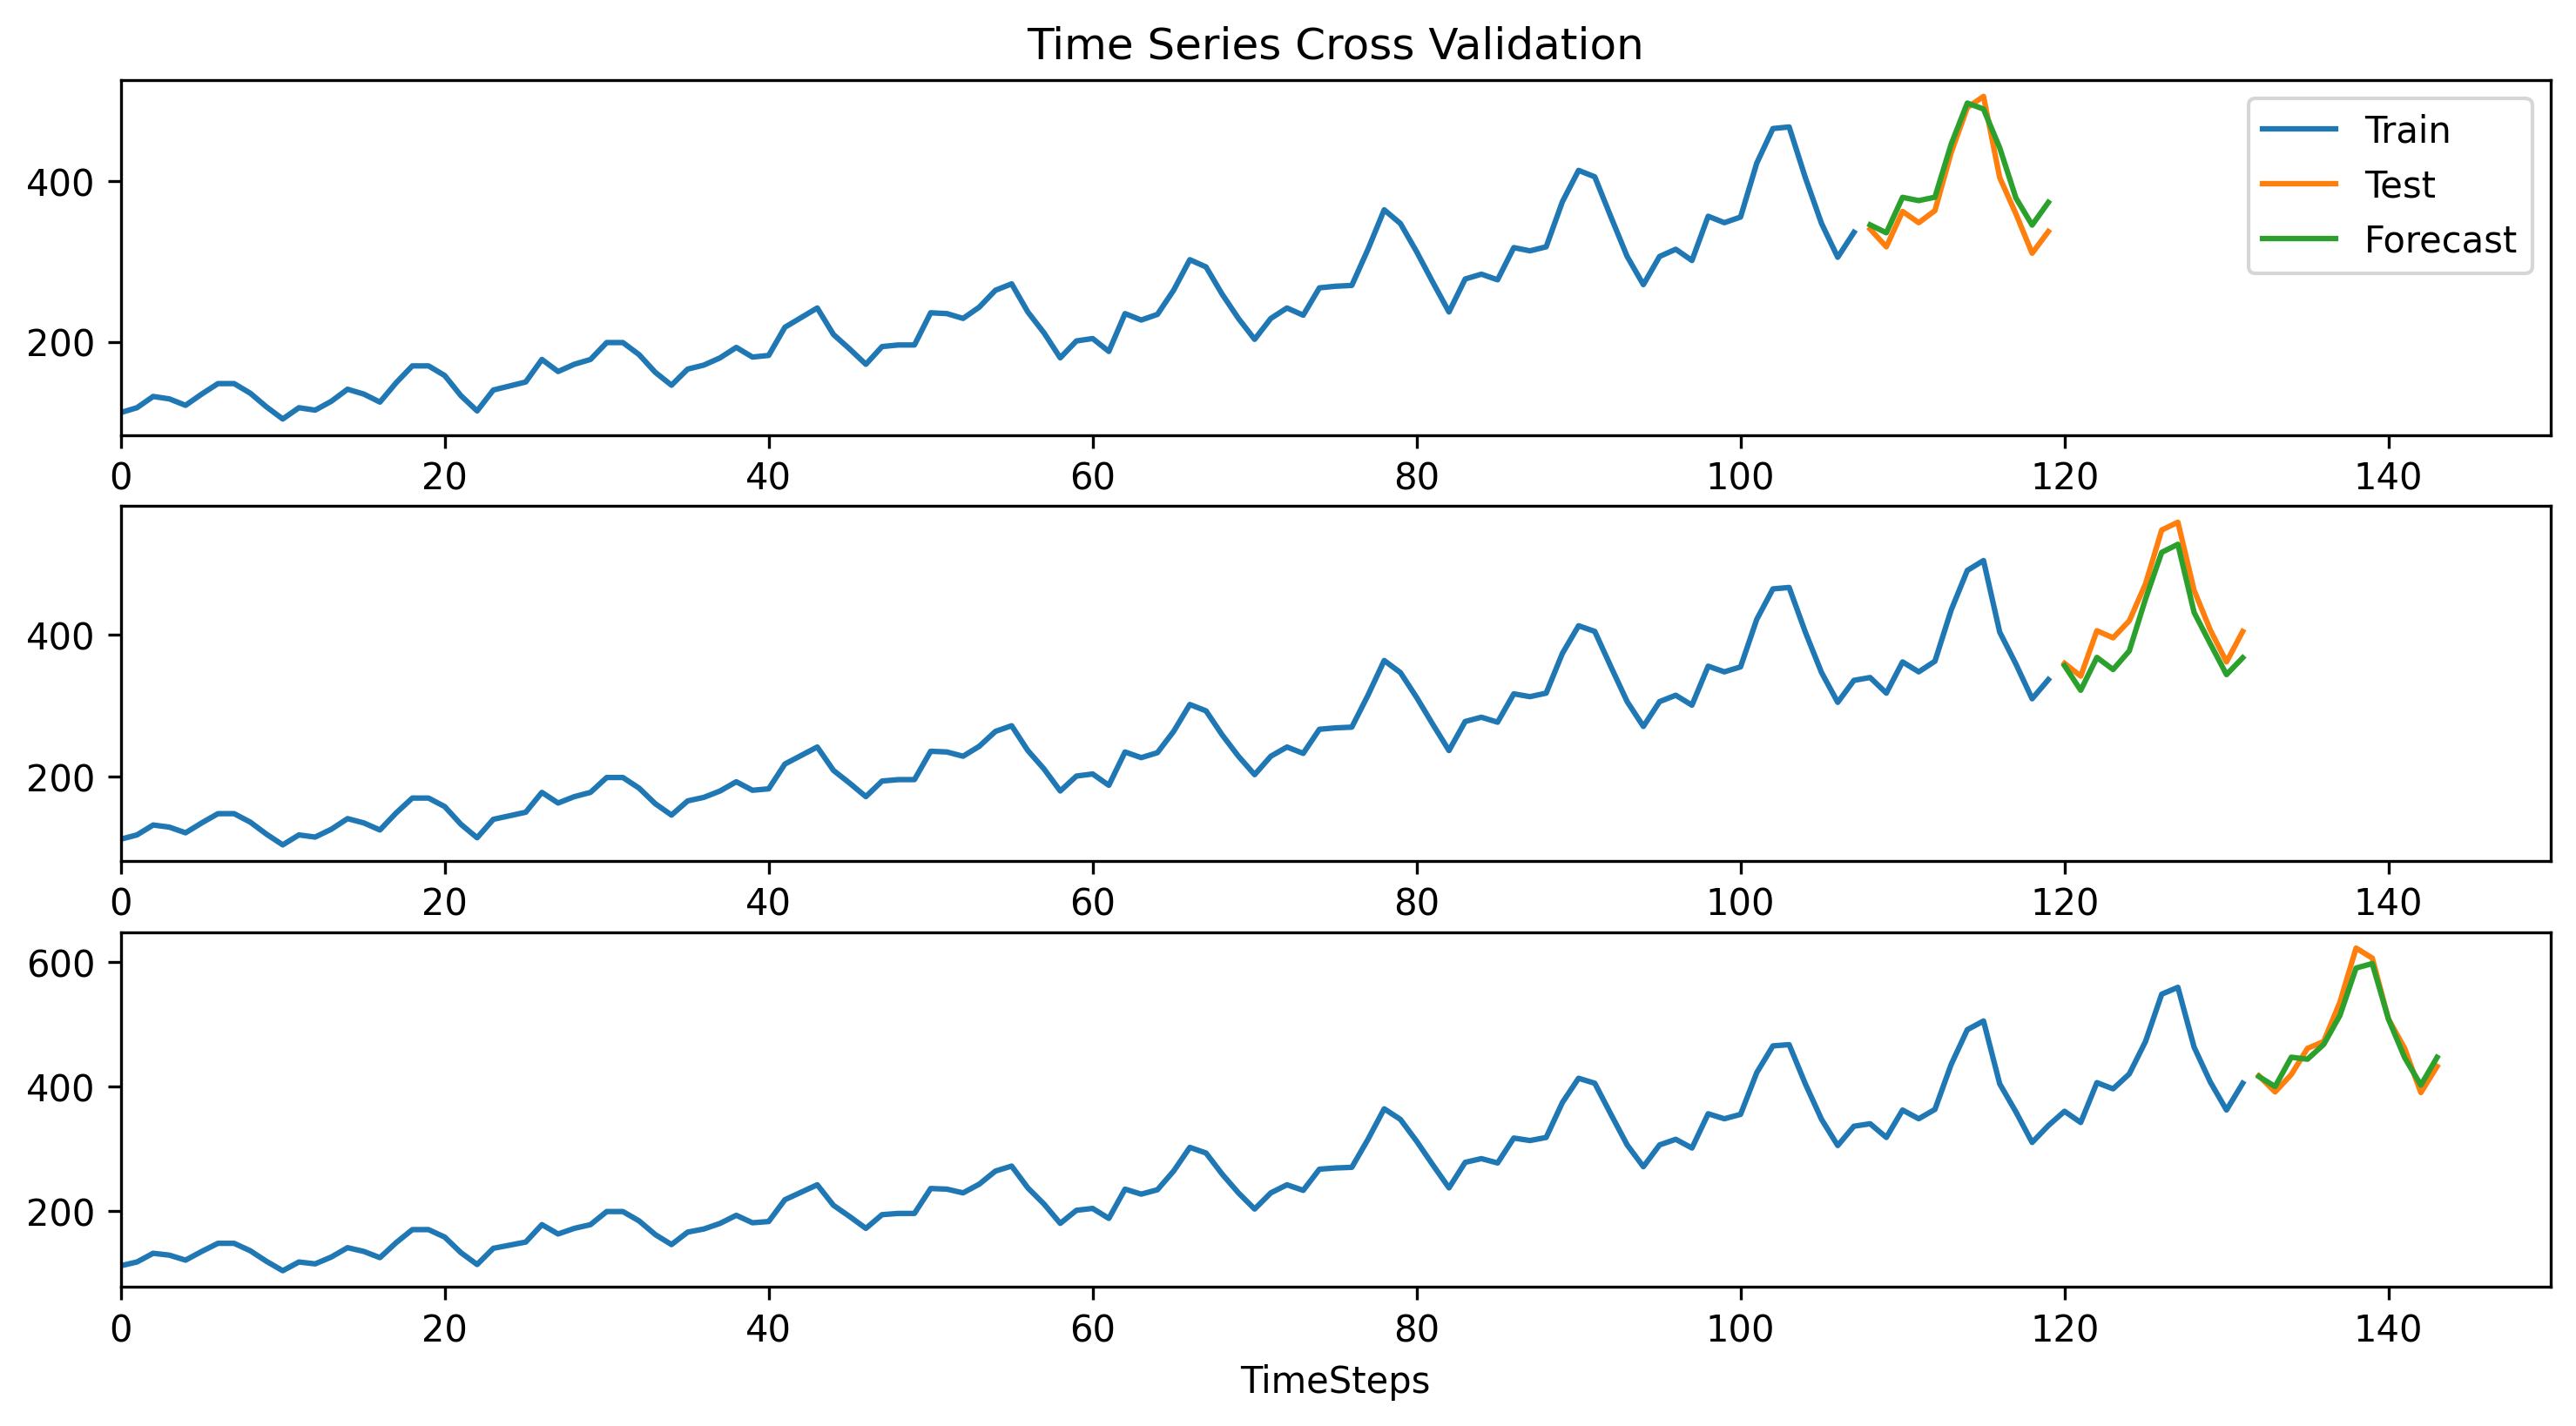
\includegraphics[scale=0.45]{notebooks/Others/img/time_series_cross_validation.png}
    \caption{Time Series Cross-Validation Example}
\end{figure}








